\chapter{Implementación y pruebas}\label{cap:implementacion}\label{ap:implementacion-detallada}

Este capítulo describe cómo se ha construido el sistema. Empieza por el entorno reproducible y
las versiones fijadas, sigue con la adquisición y el gobierno de los datos, con el backend y con
el frontend; termina con las pruebas, la verificación y el despliegue. Incluye extractos de
código representativos, todos referenciados en el texto.

\section{Entorno reproducible y dependencias}\label{sec:impl-entorno}\label{sec:datos-dependencias}

El entorno de desarrollo y de pruebas se orquesta con Docker Compose, con tres servicios de
aplicación (base de datos, backend y frontend), además de los \textit{workers} de las variantes
de recomendación que publica la web (Sección~\ref{sec:alg-publicadas}). Las dependencias se fijan a versión exacta, con
\texttt{uv} para Python y \texttt{pnpm} para Node. Sus ficheros de bloqueo se congelan en las
construcciones. Las imágenes base se fijan por resumen criptográfico. La
Tabla~\ref{tab:stack} recoge las versiones principales.

\begin{table}[htp]
\centering
\begin{tabularx}{\textwidth}{ | L{0.24\textwidth} | C{0.18\textwidth} | Y | }
    \hline
    \textbf{Componente} & \textbf{Versión} & \textbf{Papel} \\
    \hline
    Python & 3.13.7 & Lenguaje del backend y de los guiones de datos. \\
    \hline
    Django & 5.2.17 LTS & Dominio, autenticación, ORM, sesiones y migraciones. \\
    \hline
    Django REST Framework & 3.18.0 & Serialización, permisos y API. \\
    \hline
    PostgreSQL & 18.6 & Base de datos de aplicación y de pruebas de integración. \\
    \hline
    psycopg & 3.3.5 & Controlador de PostgreSQL. \\
    \hline
    Node.js & 24.13.0 & Ejecución del frontend. \\
    \hline
    Next.js & 16.3.4 & Renderizado en el servidor, rutas y metadatos. \\
    \hline
    React & 19.2.7 & Modelo de componentes. \\
    \hline
    TypeScript & 6.0.3 & Tipado estricto del frontend. \\
    \hline
    Tailwind CSS & 4.3.3 & Tokens de diseño y maquetación adaptable. \\
    \hline
\end{tabularx}
\caption{Versiones principales del entorno reproducible.}
\label{tab:stack}\label{tab:stack-resumen}
\end{table}

Toda dependencia directa nueva o cambio de versión pasa por un gate: aprobación humana
explícita, verificación de la ficha oficial del repositorio de paquetes, fijación a versión
exacta con su árbol transitivo en el fichero de bloqueo, una fila en
\texttt{docs/verification/dependency-legitimacy.md}, una fila en el gate
\texttt{check-dependencies.ps1} y una entrada en el registro de agentes. En el sistema solo
se añadieron dos dependencias directas. La primera es \texttt{requests} en la versión 2.34.2,
para el importador de IGDB. La segunda es \texttt{gunicorn} en la versión 23.0.0, como
servidor de producción de la API tras una revisión de código. Ambas se verificaron contra la
ficha oficial del índice de paquetes de Python, con su licencia, su versión mínima de
intérprete y su fecha de publicación reales.

\section{Adquisición y gobierno de datos}\label{cap:datos}

Esta sección describe de dónde salen los datos del catálogo, bajo qué licencia se usan y qué
evidencia de procedencia se conserva. El sistema integra dos fuentes de datos de catálogo. La
primera es un corpus curado de ciento cincuenta juegos procedente de Wikidata, que actúa como
la referencia citable y estable. La segunda es el catálogo a escala real procedente de IGDB,
con más de trescientas mil obras. Las dos conviven en la base de datos, indexadas por su
fuente, pero la evaluación solo consume la vista gobernada y versionada. La
Figura~\ref{fig:flujo-catalogo} recoge el recorrido completo de los datos, de las fuentes al
laboratorio.

\begin{figure}[htp]
    \centering
    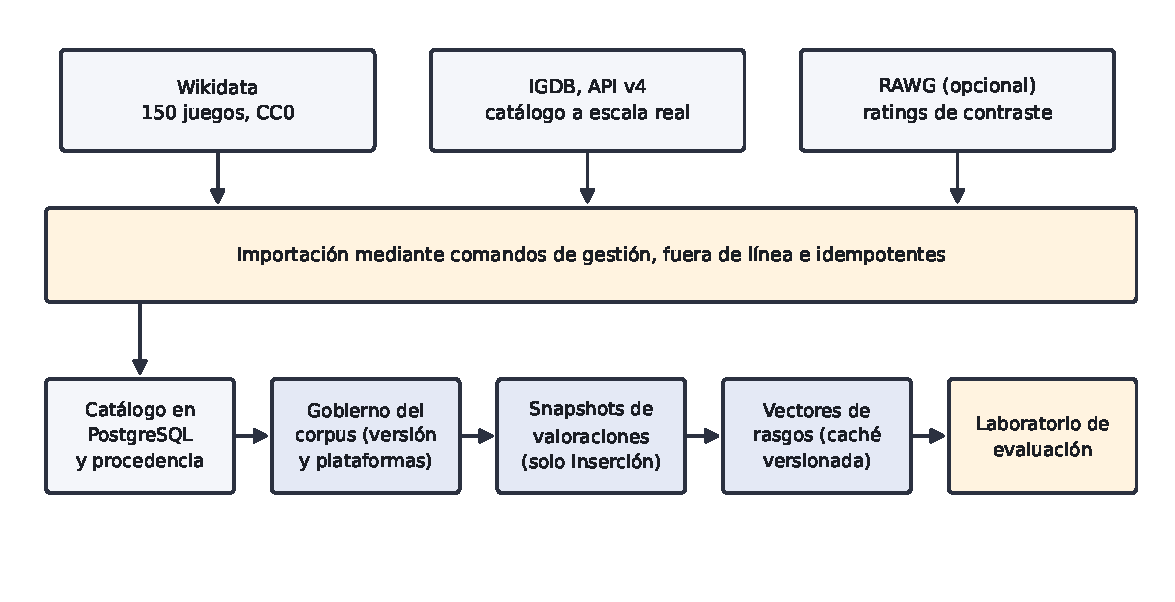
\includegraphics[width=0.9\textwidth]{figures/flujo-catalogo.pdf}
    \caption{Flujo de los datos del catálogo, desde las fuentes hasta el laboratorio de evaluación.}
    \label{fig:flujo-catalogo}
\end{figure}

\subsection{Fuentes: corpus de Wikidata y catálogo de IGDB}\label{sec:datos-wikidata}\label{sec:datos-igdb}

El corpus curado son ciento cincuenta juegos de datos estructurados de Wikidata,
publicados bajo la dedicación al dominio público \textit{Creative Commons Zero}
(CC0)~\cite{wikidata-licensing}. La adquisición se hace fuera de línea con un guion que
lanza una consulta filtrada por clase contra el punto de acceso SPARQL de Wikidata, resuelve
las subconsultas de plataforma de forma dinámica y valida la estructura y la cobertura por
época del resultado. El guion escribe el fichero \texttt{data/raw/wikidata-games.json} con su
huella SHA-256, más los manifiestos de catálogo y de recursos. El registro de decisión
ADR-003 y el documento \texttt{docs/verification/catalogue-freeze.md} conservan la consulta,
la fecha de corte en tiempo universal coordinado, la huella y la aprobación humana explícita
del corpus.

Los archivos multimedia se tratan por separado, porque no comparten la licencia de los datos
estructurados. De diecinueve archivos de Wikimedia Commons revisados uno a uno, diecisiete se
admitieron con crédito completo de autor, licencia y fuente. Los dos restantes se
sustituyeron por un marcador de reserva de primera parte~\cite{commons-reuse}. El identificador de Wikidata se
conserva solo como procedencia en \texttt{SourceRecord}, nunca como clave primaria, de modo
que la identidad del producto no queda acoplada a la fuente.

El catálogo a la escala de un producto real se construye con la API de
versión 4 de IGDB~\cite{igdb-api}. El requisito DATA-04 exige elegir la fuente mediante una
comparación documentada de cobertura, plataformas, licencia, atribución, cuotas, estabilidad
y coste. La Tabla~\ref{tab:data04} resume esa comparación, que se apoya en un sondeo
autenticado en vivo de la API ejecutado el 5 de septiembre de 2026 y en fuentes secundarias
para las otras dos opciones.

\begin{table}[htp]
\centering
\begin{tabularx}{\textwidth}{ | L{0.15\textwidth} | Y | Y | Y | }
    \hline
    \textbf{Eje} & \textbf{IGDB (elegida)} & \textbf{RAWG} & \textbf{Wikidata escalado} \\
    \hline
    Cobertura & 374.555 entradas totales, 312.418 juegos principales, medidos en vivo & Entre 350.000 y 500.000 declarados, fuente secundaria & Escasa y desigual para juegos \\
    \hline
    Plataformas & Entidad de primera clase, 220 filas & Metadatos de primera clase, fuente secundaria & Presentes pero inconsistentes \\
    \hline
    Licencia & \textit{Twitch Developer Services Agreement}, gratuita para uso comercial y no comercial & Nivel gratuito solo no comercial & CC0, la más limpia \\
    \hline
    Atribución & Estática y visible a IGDB.com & Obligatoria con enlace de vuelta en cada página & No requerida para datos CC0 \\
    \hline
    Cuotas & Sin cuota mensual; 4 peticiones por segundo & 20.000 peticiones al mes en el nivel gratuito & Sin cuota, sujeta a límites del punto de acceso \\
    \hline
    Estabilidad & API v4 estable desde 2020, respaldada por Twitch & Operador independiente, mayor riesgo & Muy estable como institución, datos de juegos volátiles \\
    \hline
    Coste & Cero & Cero dentro de la cuota & Cero \\
    \hline
\end{tabularx}
\caption{Comparación DATA-04 de fuentes para el catálogo a escala real.}
\label{tab:data04}
\end{table}

De la comparación se desprende la elección de IGDB, la única opción que combina cobertura
real, modelado de género y plataforma de primera clase, ausencia de cuota mensual y coste
cero, a cambio de una obligación de atribución continua. La frontera de categoría es
\texttt{game\_type = 0}, es decir, solo juegos principales; el contenido descargable, las
expansiones, los paquetes y los ports quedan excluidos del catálogo primario. Las portadas se
sirven por enlace directo al servidor de imágenes de IGDB, no se replican, con el marcador de
reserva de primera parte como alternativa cuando una portada falta o falla. La
regla de caché y redistribución se apoya en el texto de la propia documentación de la API,
que prefiere que el integrador almacene y sirva los datos a sus usuarios finales, texto que
se registra literalmente en el repositorio como la autorización escrita que contempla el
acuerdo general~\cite{twitch-dsa}. El corpus de Wikidata y su regla de no consultar
proveedores en tiempo de petición se conservan sin cambios; la importación de IGDB es aditiva
y se ejecuta solo desde un comando de gestión fuera de línea.

\subsection{Congelación y gobierno del corpus}\label{sec:datos-congelacion}

Una revisión humana fila a fila no es posible con cientos de miles de obras, ni es el modelo
legal correcto para las portadas de IGDB. El documento
\texttt{docs/verification/igdb-catalogue-freeze.md} congela en su lugar tres artefactos: una
huella de contenido, que es un SHA-256 sobre los pares de identificador de origen y huella
normalizada de cada registro de procedencia de IGDB, ordenados por identificador numérico;
una cobertura agregada, con el total de obras primarias, la distribución de géneros, las
plataformas más frecuentes, el histograma de año de lanzamiento y el reparto entre portada
presente y de reserva; y un manifiesto de revisión muestreada determinista de trescientos
registros, tomando uno de cada mil cuarenta y uno por orden de identificador, con datos
suficientes para una comprobación humana puntual. La Tabla~\ref{tab:freeze} recoge los
valores medidos en la carga de la base de datos de desarrollo persistente y actualizados
durante la Fase 2, el 7 de septiembre de 2026.

\begin{table}[htp]
\centering
\begin{tabularx}{\textwidth}{ | L{0.60\textwidth} | Y | }
    \hline
    \textbf{Campo} & \textbf{Valor} \\
    \hline
    Obras primarias de IGDB importadas & 312.560 \\
    \hline
    Corpus de Wikidata conservado & 150 \\
    \hline
    Total de obras en el catálogo & 312.710 \\
    \hline
    Géneros & 23 \\
    \hline
    Plataformas (Wikidata e IGDB reconciliadas) & 288 \\
    \hline
    Portadas presentes / de reserva & 268.679 / 43.804 \\
    \hline
    Fecha de primer lanzamiento poblada & aproximadamente el 75\% de las filas \\
    \hline
    Obras con valoración de usuarios de IGDB & 27.014 (13,9330\% del corpus gobernado) \\
    \hline
    Cobertura de \texttt{total\_rating} & 15,8197\% del corpus gobernado \\
    \hline
    Huella de contenido (SHA-256) & \texttt{ff3d67525c92\ldots} \\
    \hline
\end{tabularx}
\caption{Evidencia agregada de congelación de la importación de IGDB.}
\label{tab:freeze}
\end{table}

La importación se probó además sobre una base de datos desechable, donde sobrevivió a una
interrupción abrupta tras dos lotes confirmados y reanudó hasta completar sin duplicados ni
huecos. Una segunda pasada completa sobre la base ya poblada convergió de forma idempotente,
con la única diferencia de dos juegos primarios que IGDB añadió en vivo entre las dos
pasadas. La versión inmutable reutilizable de la base cargada, de noventa y tres megabytes, no se
versiona en el repositorio por decisión de ADR-006; se conserva fuera de él como vía de
restauración rápida.

La Fase 2 añadió una frontera de evaluación sobre este catálogo. El comando
\texttt{govern\_corpus} aplica las reglas D-03 de forma reversible: conserva las obras
fuente, pero marca como gobernadas las que son obras principales, tienen fecha de lanzamiento,
al menos un género y al menos una plataforma de la lista permitida de 39 plataformas. La valoración no es un criterio de
exclusión. La ejecución documentada el 7 de septiembre dejó 193.885 obras gobernadas y una versión de corpus
\texttt{2026.09.1}; el checksum, el diccionario, el informe de calidad y la muestra
determinista se conservan en \texttt{docs/verification/corpus-governance-freeze.md}. La
Tabla~\ref{tab:freeze} y las cifras de este párrafo corresponden a esa versión. El 9 de septiembre se
congeló la versión \texttt{2026.09.2}, con corte temporal en esa fecha: el catálogo visible no contiene
obras posteriores al corte, sin fecha ni contenido descargable, y deja \textbf{190.479 obras
gobernadas}. Es la versión con la que trabajan el laboratorio de evaluación y los resultados del
Capítulo~\ref{cap:resultados}, y su evidencia está en
\texttt{docs/verification/corpus-governance-2026.09.2.json}.

\subsection{Valoraciones externas y aislamiento de la evaluación}\label{sec:datos-ratings}

Durante la reimportación de IGDB se añadieron los campos \texttt{rating},
\texttt{rating\_count} y \texttt{total\_rating\_count}, además del resumen y los alias
alternativos. El campo \texttt{rating} representa la valoración de usuarios de IGDB en una
escala de 0 a 100; \texttt{total\_rating} representa la valoración agregada disponible en
IGDB. Son señales distintas y por eso se almacenan con nombres distintos. En el corte de
\texttt{2026.09.1}, la cobertura de ambos campos sobre las obras gobernadas es la que recoge
la Tabla~\ref{tab:freeze}.

El comando \texttt{snapshot\_corpus\_ratings} copia las valoraciones externas a
\texttt{CorpusRatingSnapshot} con una operación insert-only asociada a una
\texttt{corpus\_version}. Una reimportación puede actualizar los campos vivos que usa la
interfaz y producir una versión posterior, pero no modifica la versión inmutable ya
utilizada por el laboratorio. Esta separación es la condición que permite repetir una
comparación y explicar qué datos recibió.

Como fuente secundaria se probó RAWG en una ejecución acotada a 10.000 obras seleccionadas
por \texttt{rating\_count} de IGDB. La reconciliación fue determinista: primero se intentó
el slug exacto y después el título normalizado junto con el año de lanzamiento. No se aplicó
emparejamiento difuso; las filas no emparejadas se descartaron y se contabilizaron. El resultado
fue de 8.575 emparejamientos y 1.425 descartes, con 8.575 versiones inmutables de RAWG insertadas. La
cobertura nueva fue cero porque las obras seleccionadas ya tenían valoración de IGDB. RAWG se
documenta, por tanto, como contraste de procedencia, no como una fuente que haya ampliado
la cobertura del corpus.

La valoración mostrada en la ficha es una decisión de producto diferente. Puede mezclar,
con pesos limitados por la cantidad de observaciones, la valoración externa y las valoraciones
locales de las personas usuarias. El laboratorio no lee esa mezcla derivada ni el
valor mutable de \texttt{GameWork}: utiliza las versiones inmutables de la versión fijada. Esta
distinción evita que una nueva valoración de una cuenta o una reimportación cambie
retroactivamente un resultado académico.

\section{Backend}\label{sec:impl-backend}

\subsection{Comandos de gestión y del laboratorio}\label{sec:impl-comandos}

Toda tarea de datos es un comando de gestión de Django, ejecutable fuera de la petición HTTP e
idempotente. El importador de Wikidata, \texttt{import\_catalogue}, carga el corpus curado
de Wikidata. El importador de IGDB, \texttt{import\_igdb\_catalogue}, recorre la API por
lotes con un cursor de identificador reanudable: cada lote se confirma dentro de una
transacción que también escribe el cursor. Un disparador de base de datos impide que ese
cursor retroceda, de modo que una ejecución interrumpida siempre reanuda hacia delante desde
el progreso real. La cadena de arranque del despliegue encadena la migración y la importación del
catálogo, como describe la Sección~\ref{cap:despliegue}.

La gobernanza y las valoraciones externas de la Sección~\ref{cap:datos} se ejecutan con
\texttt{govern\_corpus}, \texttt{snapshot\_corpus\_ratings} y \texttt{enrich\_rawg\_ratings}, que
trabaja por lotes con \textit{backoff} ante respuestas transitorias.
\texttt{backfill\_game\_aliases} reconstruye los alias normalizados para que la búsqueda sea útil
sobre el catálogo real.

El protocolo se carga desde \texttt{docs/methodology/protocol.json}. Los módulos de la
aplicación \texttt{evaluation} que describe la Sección~\ref{sec:dis-laboratorio} se
implementan con funciones deliberadamente pequeñas y explícitas.
\texttt{evaluation/protocol.py} rechaza una rejilla con más de 24 configuraciones y distingue
un protocolo todavía no consumido de una prueba ya ejecutada. \texttt{evaluation/metrics.py} no
delega la definición de P@K, R@K, nDCG@K o MAP@K en una librería externa.
\texttt{evaluation/splits.py} deriva la semilla del protocolo y del usuario, para que el orden
de las filas en la base de datos no altere la obra retenida.

\subsection{Vistas, búsqueda y filtrado}\label{sec:impl-vistas}\label{sec:impl-busqueda}

La configuración de DRF fija la autenticación por sesión como única clase de autenticación,
de modo que no queda habilitada ninguna vía de autenticación básica sin límite de ritmo. Los
límites de ritmo de las vistas anónimas de mayor coste son: cinco registros
por hora, diez intentos de acceso por minuto, treinta consultas de perfil por minuto
y ciento veinte búsquedas de catálogo por minuto. El número de proxies de confianza se lee de
una variable de entorno, con valor cero en local, para que el límite de ritmo por dirección
se agrupe correctamente detrás del proxy del mismo origen.

La búsqueda del catálogo es tolerante: primero coincidencia exacta, después por prefijo y por
último por similitud de trigramas para erratas pequeñas, siempre sobre el índice de alias
normalizados y sin ninguna llamada externa. Sobre ese resultado se cruzan los filtros de
plataforma, género, año y nota mínima. Una lista fija de claves de ordenación se traduce a un
\texttt{order\_by} determinista con desempate por identificador canónico. El texto de
ordenación que envía el cliente nunca se interpola: una clave desconocida produce un error
acotado antes de tocar el ORM. El Extracto de código~\ref{cod:sort} muestra esa lista de
ordenaciones permitidas.

\begin{lstlisting}[language=Python, caption={Lista fija de ordenaciones del catálogo, con desempate por identificador canónico (\texttt{apps/api/catalogue/search.py}).}, label={cod:sort}, captionpos=b]
# Cada clave resuelve a una tupla de argumentos de order_by que SIEMPRE
# termina en canonical_slug, de modo que todo orden es total y estable
# entre llamadas. Nada derivado de la entrada del cliente llega a este
# diccionario: una clave no reconocida lanza un error antes de construir
# la consulta.
SORT_ORDERS = {
    "title_asc": ("original_title", "canonical_slug"),
    "title_desc": ("-original_title", "canonical_slug"),
    "release_newest": (F("first_release_date").desc(nulls_last=True), "canonical_slug"),
    "release_oldest": (F("first_release_date").asc(nulls_last=True), "canonical_slug"),
    "rating_desc": (F("total_rating").desc(nulls_last=True), "canonical_slug"),
}
\end{lstlisting}

\subsection{Recomendadores en la aplicación}\label{sec:impl-heuristico}

La aplicación publica tres variantes del laboratorio (Sección~\ref{sec:alg-publicadas}), cada una
servida por su proceso trabajador. Además, el método de referencia \texttt{rank\_random\_v1} es el suelo de
comparación. Selecciona con
\texttt{random.Random(seed)} sobre los candidatos gobernados que no aparecen en la biblioteca
de la persona usuaria. Ordenar previamente los identificadores y guardar una huella de la
semilla, los candidatos y el resultado hace que la misma entrada produzca exactamente el
misma clasificación.

El modelo de contenido que usan los algoritmos, descrito en la
Sección~\ref{cap:algoritmos}, se apoya en \texttt{WorkFeatureVector}, una caché versionada y
no un modelo entrenado, que \texttt{rebuild\_feature\_vectors} rellena de forma idempotente. El
perfil de usuario se construye con los pesos de actividad descritos a continuación, y la
valoración se mantiene fuera del vector para poder estudiarla como una señal independiente.

\begin{samepage}
La interfaz de recomendaciones solo muestra las tres variantes del laboratorio publicadas:
\texttt{content-cbf-weighted-v1}, \texttt{content-cbf-mmr-pop-v1} y \texttt{recency-v1}.
Cada entrada de biblioteca aporta un peso de actividad a las etiquetas curadas de su obra,
según la fórmula del Extracto de código~\ref{cod:heuristico}. Un refactor posterior extrajo ese
cálculo al módulo \texttt{apps/api/recommendations/\_weights.py}, para que las variantes de
contenido y la construcción del perfil reutilicen una única definición en lugar de copiarla. La
contribución de la valoración no es lineal, como explica la Sección~\ref{cap:algoritmos}; sin
actividad suficiente, las variantes aplican sus reglas declaradas de arranque en frío.

\begin{lstlisting}[language=Python, basicstyle=\small\ttfamily, caption={Cálculo del peso de actividad de una entrada de biblioteca.}, label={cod:heuristico}, captionpos=b]
# Pesos compartidos por los perfiles de contenido.
# Una obra abandonada no aporta evidencia positiva.
_STATUS_WEIGHTS = {
    "completed": 3.0,
    "playing": 2.0,
    "pending": 1.0,
    "abandoned": 0.0,
}

# La intensidad crece de forma no lineal con la valoracion.
_RATING_DIVISOR = 10
RATING_INTENSITY_POWER = 2.0

def _rating_intensity(rating_half_steps):
    if rating_half_steps is None:
        return 0.0
    normalised = max(
        0.0,
        min(1.0, rating_half_steps / _RATING_DIVISOR),
    )
    return normalised ** RATING_INTENSITY_POWER

def _entry_weight(status, rating_half_steps):
    status_weight = _STATUS_WEIGHTS.get(status or "", 0.0)
    return status_weight + _rating_intensity(rating_half_steps)
\end{lstlisting}
\end{samepage}

\clearpage
\section{Frontend}\label{sec:impl-frontend}\label{sec:impl-rutas}\label{sec:impl-i18n}\label{sec:impl-proxy}

\begin{samepage}
La parte cliente usa el enrutador de aplicación de Next.js, con un segmento de idioma en la raíz de
la ruta. Las rutas del sistema son la página de inicio, el catálogo, el detalle de un
juego, la colección, las amistades, el perfil propio, el perfil de un amigo, las fuentes, el acceso, el registro y las
recomendaciones. Los componentes reutilizables son los que fija el contrato de diseño de la
Sección~\ref{sec:dis-ui}, además del armazón de la aplicación con su barra de navegación. Las páginas de solo lectura se renderizan en el servidor; los controles de biblioteca
son componentes de cliente que llaman a la API del mismo origen. Las
Figuras~\ref{fig:catalogo} y~\ref{fig:coleccion} muestran el catálogo con sus filtros y la
colección de la persona usuaria.
\end{samepage}

\begin{figure}[H]
    \centering
    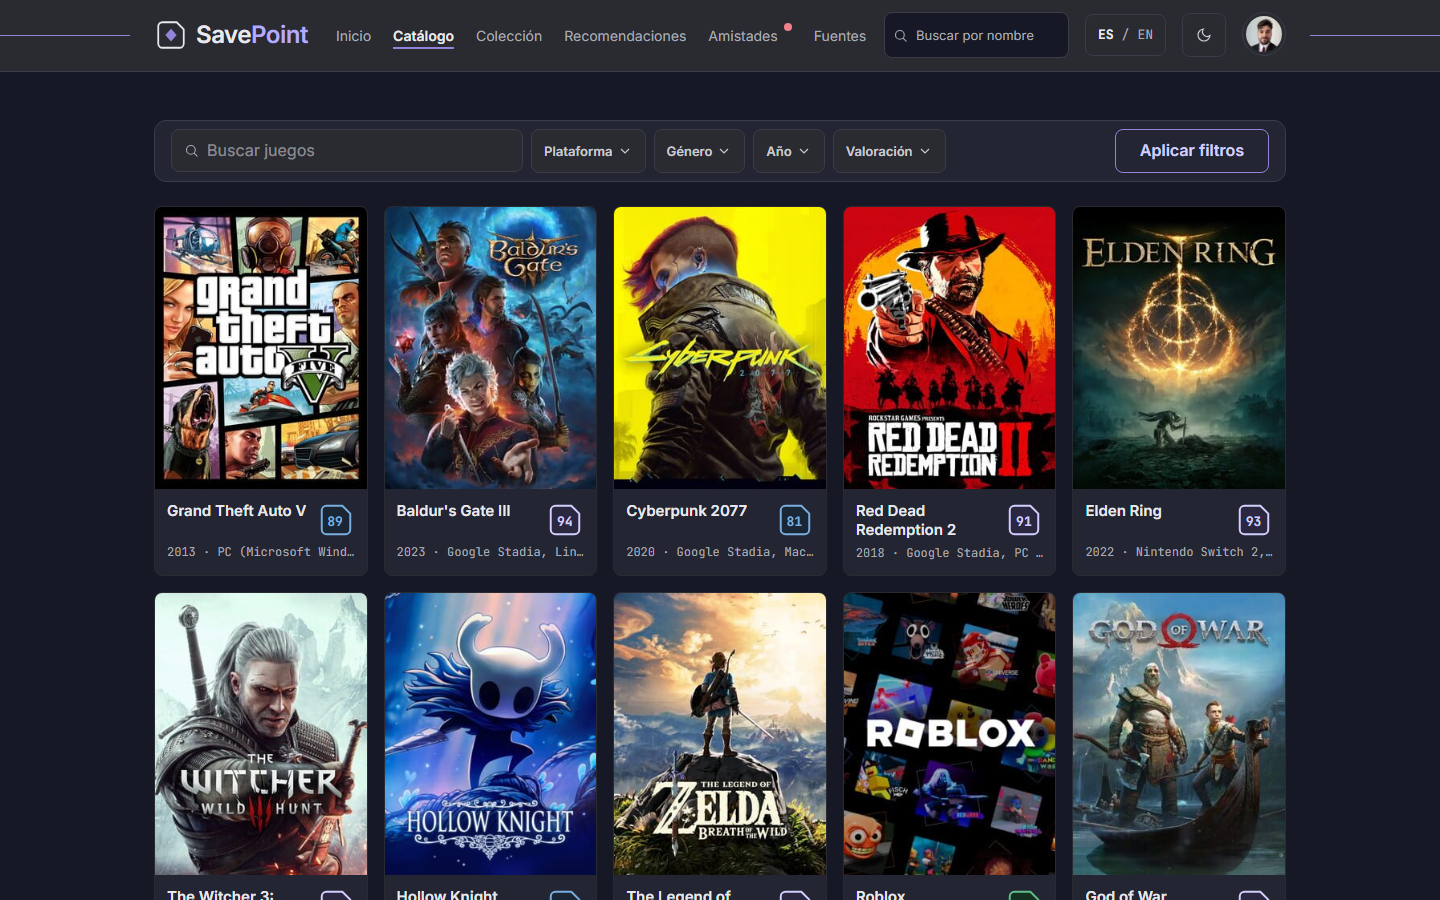
\includegraphics[width=0.85\textwidth]{figures/02-catalogo-oscuro.png}
    \caption{Catálogo con tema oscuro, búsqueda y filtros por plataforma, género, año y valoración. Fuente: captura del proyecto.}
    \label{fig:catalogo}
\end{figure}

\begin{figure}[H]
    \centering
    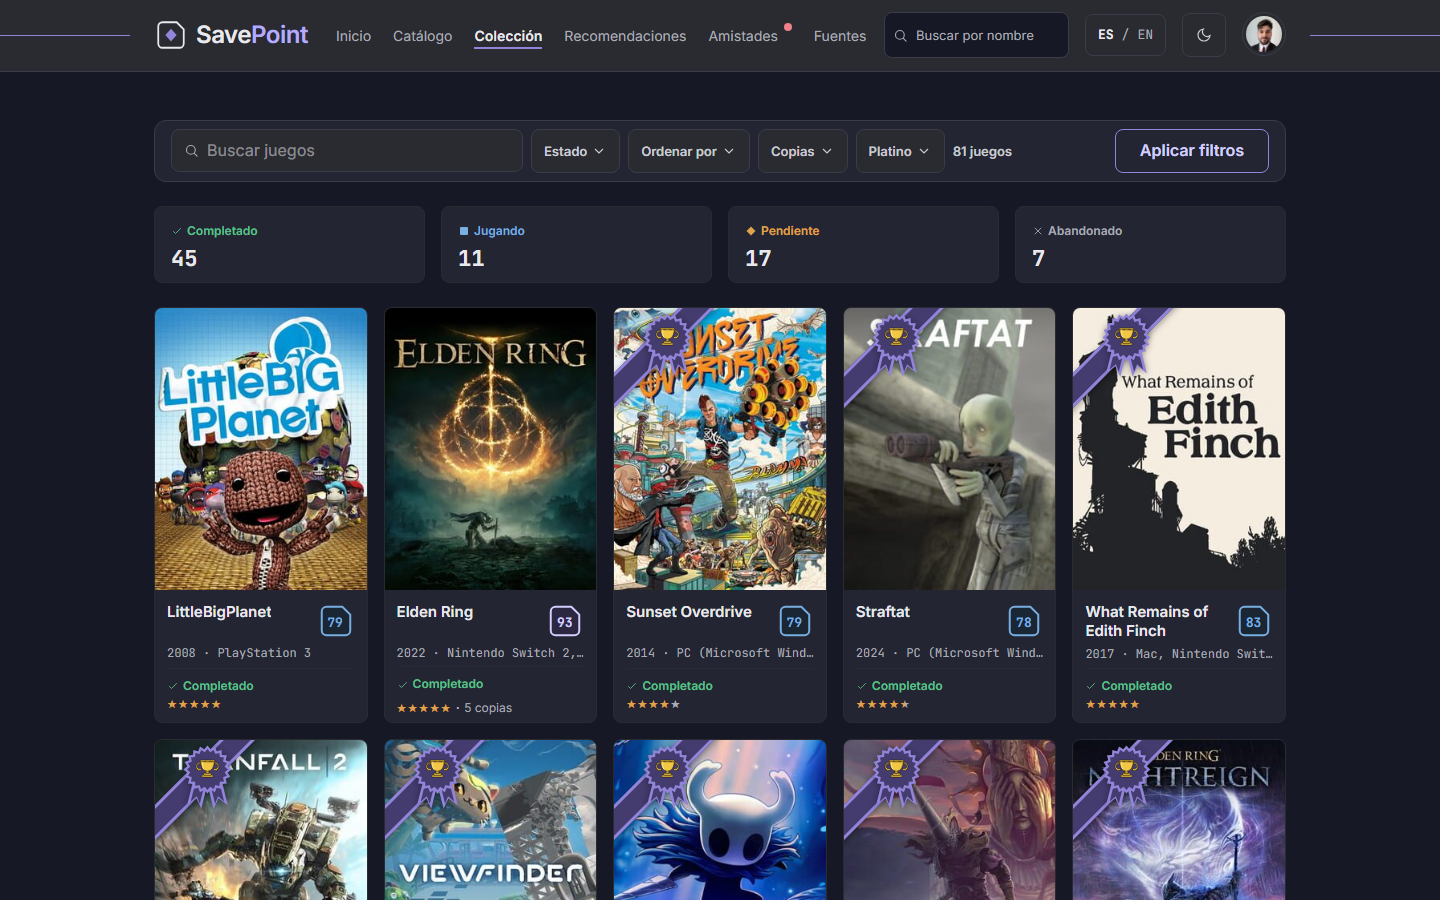
\includegraphics[width=0.85\textwidth]{figures/05-coleccion-oscuro.png}
    \caption{Colección de la persona usuaria con tema oscuro, con el estado y la valoración de cada juego. Fuente: captura del proyecto.}
    \label{fig:coleccion}
\end{figure}

La interfaz está disponible en español y en inglés. Los textos viven en diccionarios por
idioma. Una prueba de paridad falla si una clave existe en un idioma pero no en el otro, de
modo que ninguna cadena queda sin traducir.

La reescritura del lado del servidor que describe la Sección~\ref{sec:dis-sesion} reenvía las
rutas bajo \texttt{/api/} y la ruta de chequeo de salud hacia el backend, con el destino tomado
de una variable de entorno visible únicamente en el servidor. El Extracto de
código~\ref{cod:proxy} la muestra.

\begin{lstlisting}[language=javascript, caption={Reescritura del mismo origen hacia el backend (\texttt{apps/web/next.config.ts}).}, label={cod:proxy}, captionpos=b]
// El navegador solo habla con este origen de Next.js: las cookies de
// sesion y CSRF que fija Django siguen siendo del mismo origen y no hace
// falta ninguna configuracion de CORS con credenciales. API_PROXY_TARGET
// solo existe en el entorno de servidor, nunca como variable NEXT_PUBLIC_.
async rewrites() {
  return [
    { source: "/api/:path*", destination: `${API_PROXY_TARGET}/api/:path*/` },
    { source: "/health/", destination: `${API_PROXY_TARGET}/health/` },
  ];
}
\end{lstlisting}

Las Figuras~\ref{fig:recomendaciones-estanterias}
y~\ref{fig:recomendaciones-detallada} muestran las dos vistas de recomendaciones disponibles
en el proyecto, junto a la portada ya presentada en la Figura~\ref{fig:ui-claro}; son capturas
de interfaz, no evidencia de calidad de clasificación ni de resultados experimentales.

\begin{figure}[H]
\centering
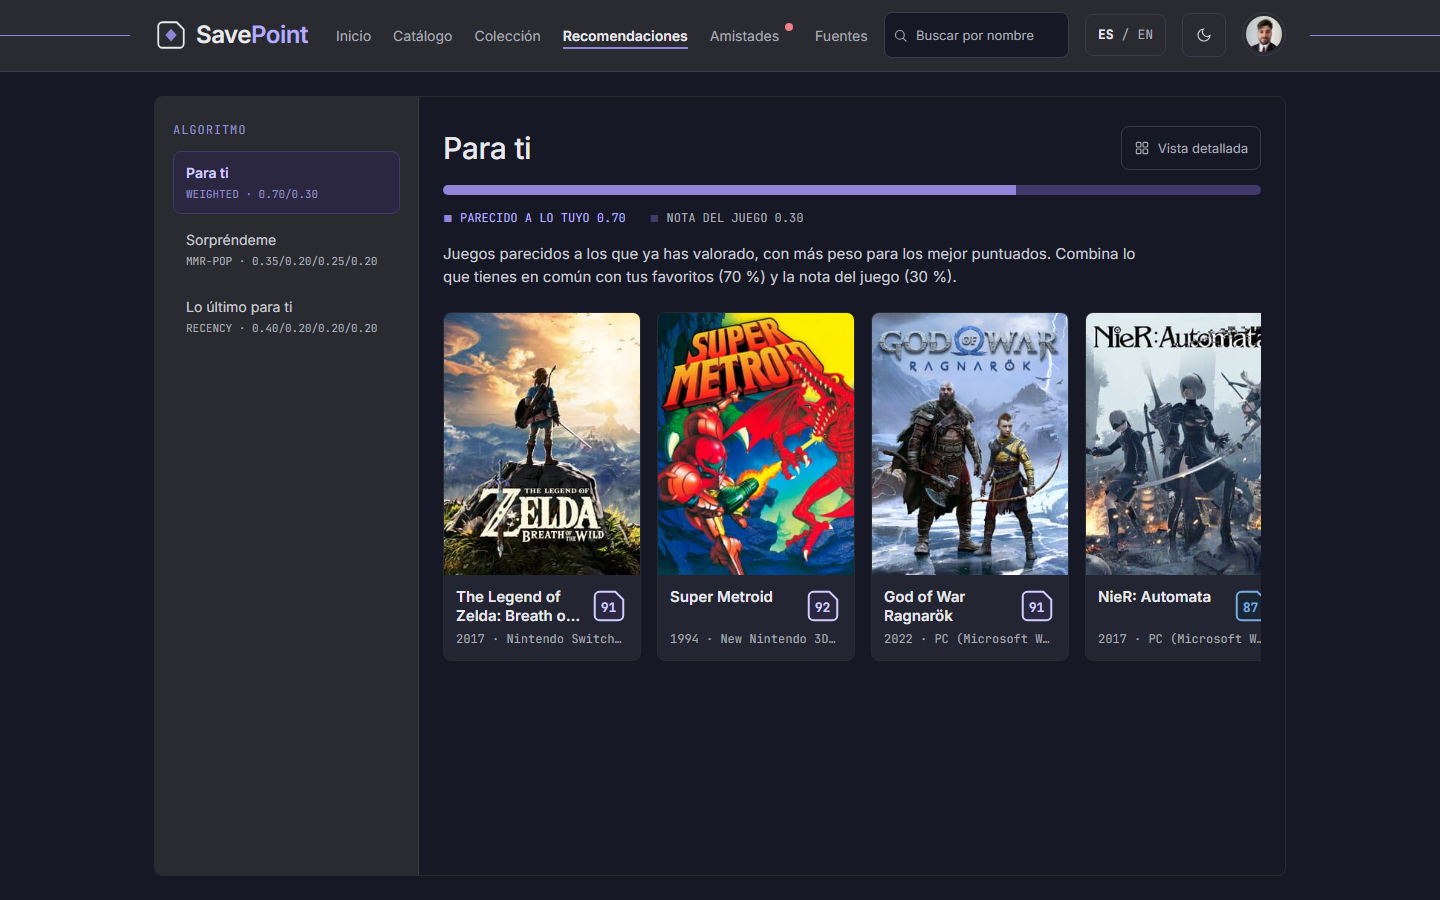
\includegraphics[width=0.82\textwidth]{figures/06-recomendaciones-estanterias-oscuro.png}
\caption{Vista de recomendaciones organizada por estanterías, con tema oscuro. Fuente: captura del proyecto.}
\label{fig:recomendaciones-estanterias}
\end{figure}

\begin{figure}[H]
\centering
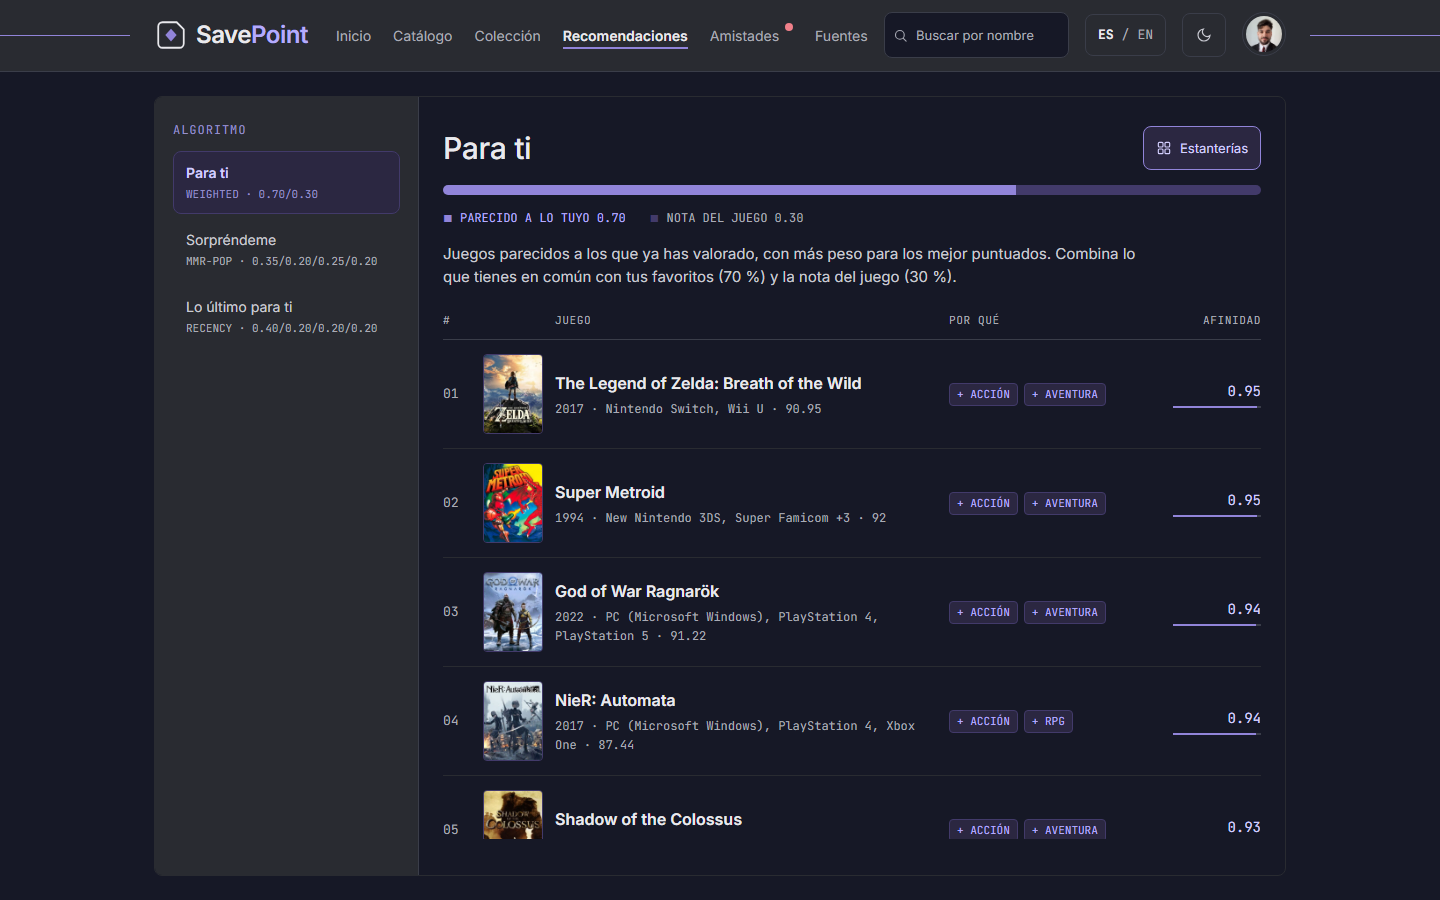
\includegraphics[width=0.82\textwidth]{figures/07-recomendaciones-detallada-oscuro.png}
\caption{Vista detallada de recomendaciones, con las señales de afinidad y tema oscuro. Fuente: captura del proyecto.}
\label{fig:recomendaciones-detallada}
\end{figure}

El módulo social y de personalización se apoya en tres pantallas. La página de amistades
(Figura~\ref{fig:amistades}) reúne en tres columnas la búsqueda por nombre de usuario exacto
y la lista de amistades, el perfil de la persona elegida, con sus favoritos y un resumen de
su colección, y las notificaciones de solicitudes y de recomendaciones, que pueden aceptarse,
rechazarse o responderse. La página de perfil propio (Figura~\ref{fig:perfil}) organiza los
ajustes en cinco pestañas: cuenta, privacidad, preferencias, conexiones y seguridad. La
primera permite editar el nombre completo, la biografía, la foto, la portada y los favoritos,
y cambiar una única vez el nombre de usuario. El acceso (Figura~\ref{fig:acceso})
y el registro (Figura~\ref{fig:registro}) son los únicos formularios abiertos a visitantes.

\begin{figure}[H]
\centering
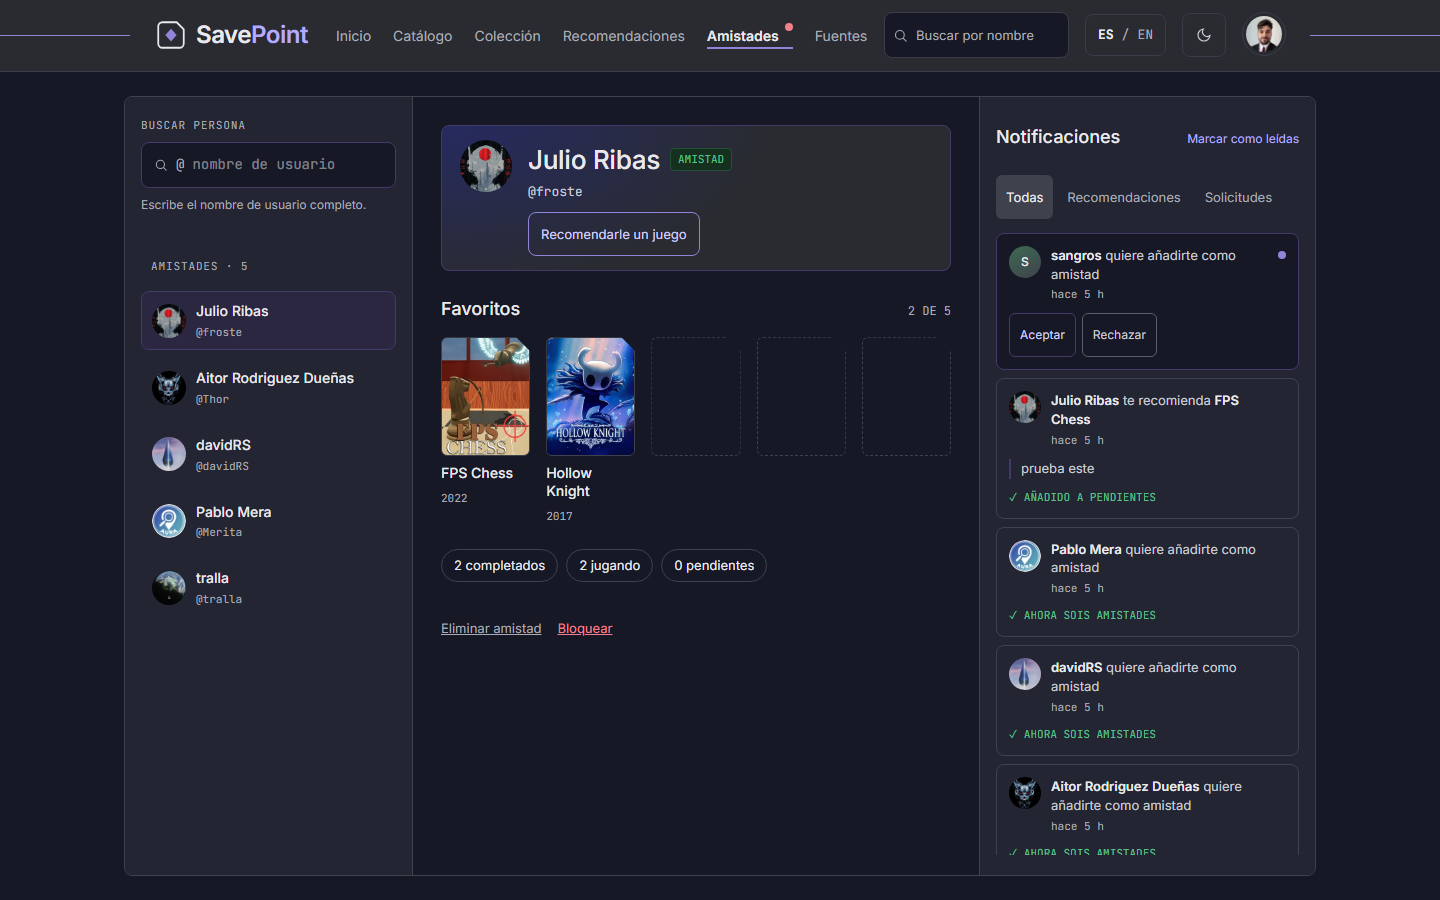
\includegraphics[width=0.85\textwidth]{figures/09-amistades-oscuro.png}
\caption{Página de amistades con tema oscuro: amistades, perfil de la persona elegida y notificaciones. Fuente: captura del proyecto.}
\label{fig:amistades}
\end{figure}

\begin{figure}[H]
\centering
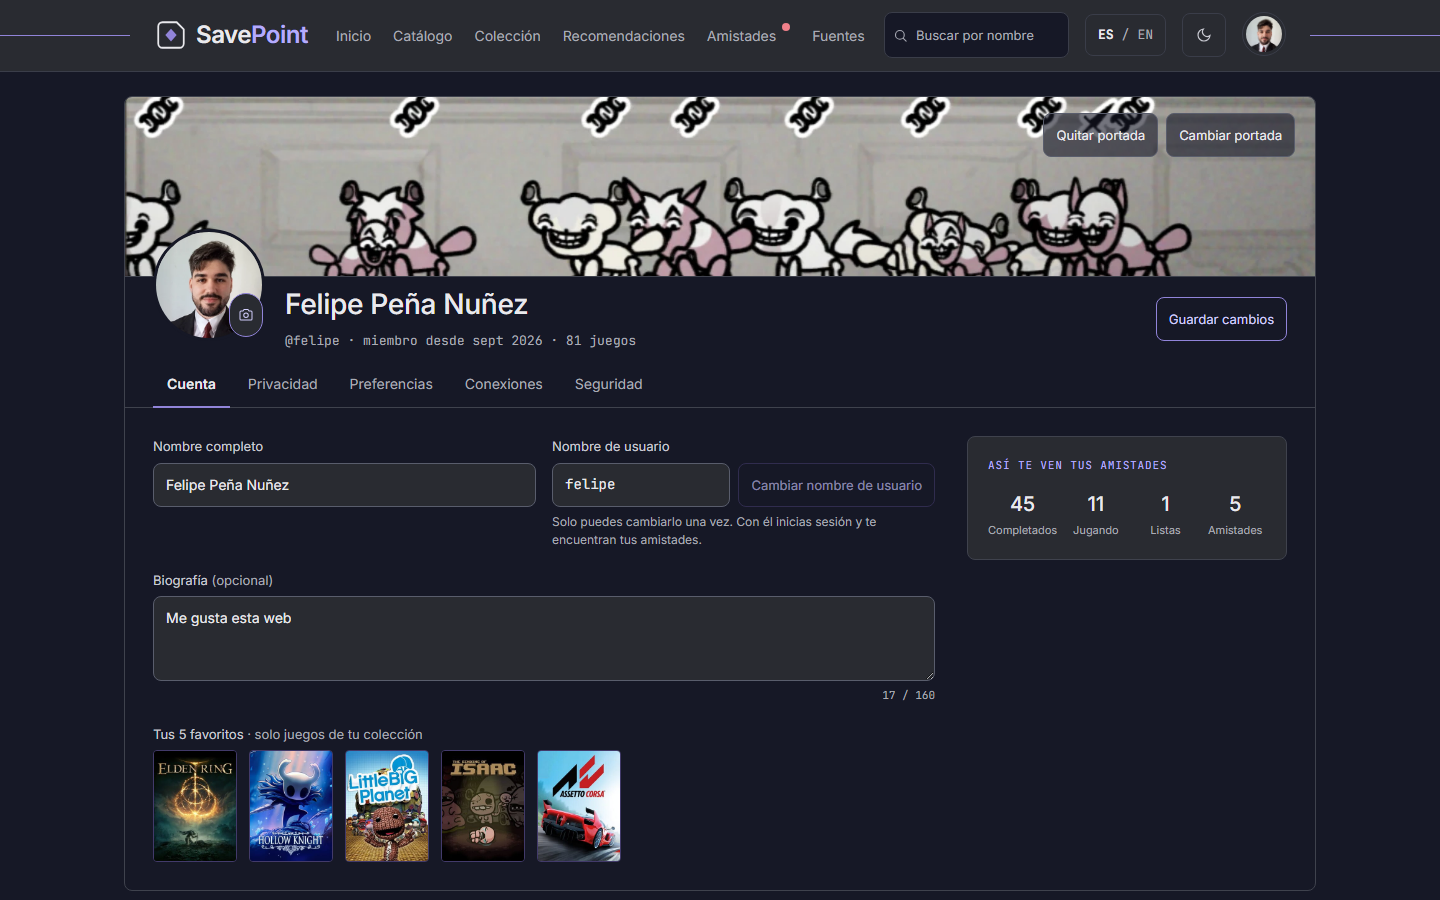
\includegraphics[width=0.85\textwidth]{figures/10-perfil-oscuro.png}
\caption{Perfil propio, pestaña de cuenta, con tema oscuro. Fuente: captura del proyecto.}
\label{fig:perfil}
\end{figure}

\begin{figure}[H]
\centering
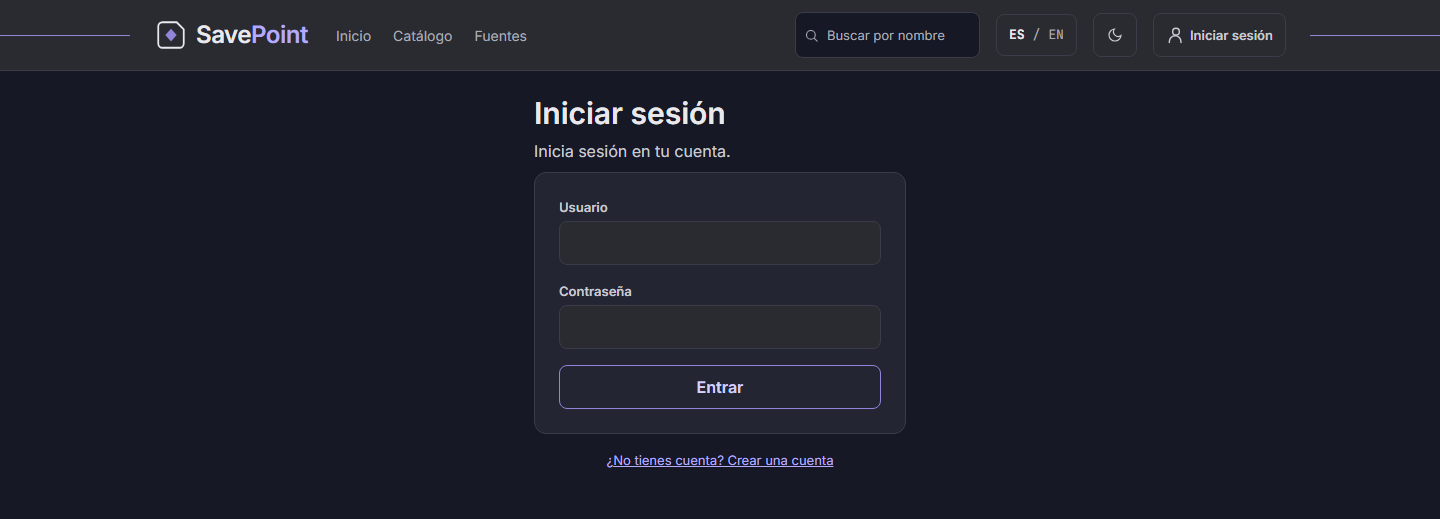
\includegraphics[width=0.85\textwidth]{figures/06-iniciar-sesion-oscuro.png}
\caption{Página de acceso con tema oscuro. Fuente: captura del proyecto.}
\label{fig:acceso}
\end{figure}

\begin{figure}[H]
\centering
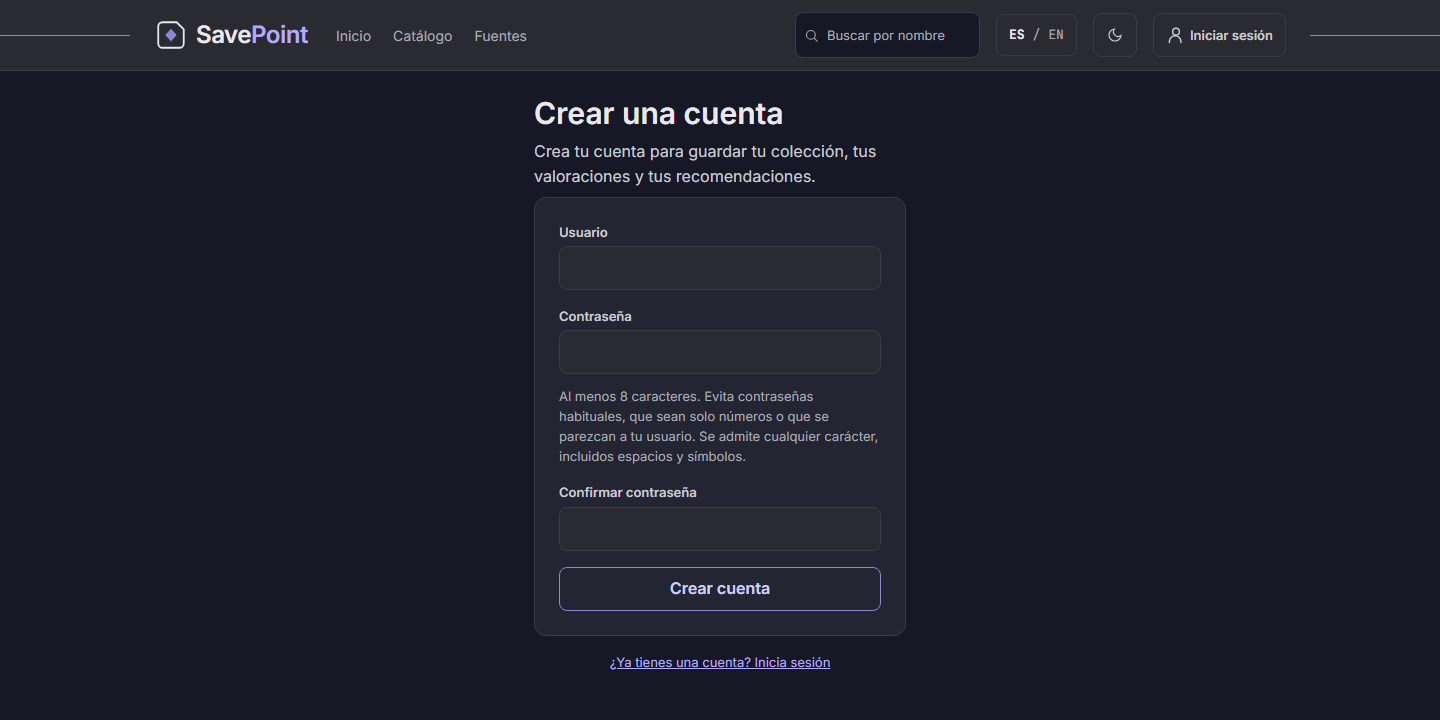
\includegraphics[width=0.85\textwidth]{figures/07-registro-oscuro.png}
\caption{Página de registro con tema oscuro. Fuente: captura del proyecto.}
\label{fig:registro}
\end{figure}

\section{Pruebas y verificación}\label{cap:pruebas}\label{sec:pru-estrategia}

La verificación combina pruebas de backend contra PostgreSQL real (unitarias e integración en
una única suite \texttt{pytest}, sin separarlas en conteos independientes), pruebas de
frontend con Vitest y un recorrido de navegador con Playwright que integra los casos de
accesibilidad mediante \texttt{axe}, sin un conteo aislado solo de accesibilidad. El cierre de
evidencia de la Fase 7, ejecutado el 14 de septiembre de 2026 y registrado en
\texttt{docs/verification/phase-07-launch-gate.md} y en \texttt{07-VERIFICATION.md}, deja como
última regresión completa 736 pruebas de backend, 70 de frontend y 56 de navegador, las tres
en verde y sin omitidas. Tras los cambios posteriores de interfaz y del módulo social, el 4 de octubre de 2026 se repitieron las suites de backend y de frontend: 773 pruebas de backend y 66 de frontend, todas en verde. El recorrido de navegador no se repitió después de esos cambios. Las evidencias de seguridad, migraciones, privacidad, importación y
exportación se citan desde \texttt{docs/verification/}.

La estrategia combina cuatro niveles. Las pruebas unitarias y de integración del backend se
ejecutan con \texttt{pytest} contra una instancia real de PostgreSQL 18.6, sin sustituirla
por una base en memoria, porque el sistema depende de restricciones, transacciones y búsqueda
de trigramas que solo se comportan igual sobre el motor real. Las pruebas del frontend usan
\texttt{vitest} para la lógica y los componentes, con una prueba de paridad de claves de
traducción. Las pruebas de extremo a extremo (E2E) usan Playwright sobre un navegador real, con la
biblioteca \texttt{axe} para las comprobaciones automáticas de accesibilidad frente a las
Pautas de Accesibilidad para el Contenido Web (WCAG) 2.2~\cite{wcag22}. Por último, una
prueba de humo se ejecuta contra la URL pública desplegada y rechaza un despliegue con la
revisión equivocada, tráfico entre orígenes inesperado o peticiones fallidas.

Las comprobaciones de \texttt{axe} cubren el catálogo, el detalle, el registro, las
recomendaciones, la página de inicio, el acceso y las fuentes, en escritorio a 1280 por 800
píxeles y en móvil a 375 por 812 píxeles.

\subsection{Verificación de los datos y del laboratorio}\label{sec:pru-fase2}

La verificación de los datos y del laboratorio se dividió en dos grupos. El primero comprobó que los datos y
sus contratos eran correctos: 70 pruebas del catálogo cubrieron la importación de campos de
valoración, las versiones inmutables de solo inserción y la reconciliación determinista de RAWG; 54 pruebas de
la aplicación \texttt{evaluation} cubrieron el cargador de protocolo, las particiones y las
métricas. El segundo comprobó las primitivas de recomendación: 48 pruebas cubrieron el
método de referencia aleatorio, el coseno, los vectores de contenido, el perfil de usuario, la caché
\texttt{WorkFeatureVector} y el cálculo del perfil de valoración por género.

Las propiedades relevantes se verificaron con casos pequeños y respuestas conocidas. El
método de referencia aleatorio devuelve el mismo orden para la misma semilla, no devuelve obras de la
biblioteca y no sale del corpus gobernado. La similitud coseno queda acotada entre cero y
uno, es exactamente uno para vectores iguales no nulos y vale cero para vectores ortogonales
o sin norma. Las métricas se comparan con cálculos manuales, mientras que la partición rechaza
conjuntos de entrenamiento, validación y prueba que no sean disjuntos y completos.

La prueba de datos a escala también dejó una evidencia reproducible. El enriquecimiento RAWG
se ejecutó en 18 lotes y una repetición de un lote ya procesado insertó cero versiones inmutables
adicionales. La huella de \texttt{GameWork.rating} permaneció idéntica antes y después, lo
que demuestra que el enriquecimiento no muta el valor vivo del catálogo. Esta evidencia
prueba integridad e idempotencia; no prueba que RAWG haya mejorado la calidad de las
recomendaciones.

Las tablas de precisión, recall, nDCG y MAP de la comparación completa, con las 16 variantes evaluadas, sus contrastes de significación estadística y sus amenazas a la validez, se presentan en el Capítulo~\ref{cap:resultados}.

\subsection{Gates de evidencia y verificación independiente}\label{sec:pru-gates}\label{sec:pru-verificacion-fase}

Además de las pruebas, el repositorio tiene gates deterministas que protegen la evidencia. El
gate \texttt{check-secrets.ps1} escanea el árbol de Git, los paquetes de construcción, las
capas de las imágenes y los registros capturados en busca de cadenas con forma de credencial,
y se autoverifica primero contra señuelos sintéticos. El gate \texttt{check-evidence.ps1}
valida el registro de agentes descrito en la Sección~\ref{sec:met-ledger}, y el gate
\texttt{check-dependencies.ps1} comprueba la lista permitida de dependencias de la
Sección~\ref{sec:impl-entorno}. Los gates \texttt{verify-igdb-*.ps1} comprueban el contenido del
registro de decisión de IGDB, la evidencia del sondeo y la ejecución de importación sobre una
base de datos fresca.

Cada incremento del sistema se sometió a la verificación independiente de su objetivo que
describe la Sección~\ref{sec:met-agentes}, que comprueba el código contra los criterios de
éxito en lugar de leer los resúmenes de plan. El recorrido vertical
inicial se verificó con cinco de cinco criterios de éxito, con dos elementos manuales de
accesibilidad aceptados como limitaciones nombradas: el reflujo al cuatrocientos por ciento
de zoom y una pasada con lector de pantalla. El catálogo a escala real, el rediseño de la
interfaz y los recomendadores se verificaron con cuatro de cuatro criterios. La Tabla~\ref{tab:criterios} resume esos criterios.

\begin{table}[htp]
\centering
\begin{tabularx}{\textwidth}{ | C{0.12\textwidth} | Y | C{0.19\textwidth} | }
    \hline
    \textbf{Criterio} & \textbf{Enunciado} & \textbf{Veredicto} \\
    \hline
    SC1 & Catálogo a escala real con fuente IGDB, con licencia, atribución y procedencia documentadas. & Verificado \\
    \hline
    SC2 & Ordenar y filtrar el catálogo por plataforma, género y otros metadatos. & Verificado \\
    \hline
    SC3 & La interfaz se lee como un producto de catalogación profesional. & Verificado \\
    \hline
    SC4 & Página de recomendaciones por géneros según la actividad propia, distinta de la recomendación de referencia por popularidad. & Verificado \\
    \hline
\end{tabularx}
\caption{Criterios de éxito verificados y su veredicto.}
\label{tab:criterios}
\end{table}

El criterio SC3, la calidad visual de producto, se cerró con la aprobación final. Empezó
como aprobación anticipada condicional, mientras se estaba desconectado. Quedó
confirmada sin condiciones tras una revisión remota de dieciocho capturas del entorno local
que cubrían las cuatro superficies principales en escritorio y en móvil, ambos temas y una
segunda cuenta con colección vacía como prueba visual de independencia.

\subsection{Revisión de código}\label{sec:pru-revision}\label{sec:pru-post-cierre}\label{sec:pru-lectura}

Ya con el sistema completo, el revisor de código de la Sección~\ref{sec:met-agentes} examinó
todo el árbol con una postura adversarial de búsqueda de defectos.
La revisión encontró dieciséis hallazgos, cuya distribución por severidad recoge la
Tabla~\ref{tab:hallazgos}. Se autorizó aplicar la totalidad de los hallazgos, que se
corrigieron en cinco tandas confirmadas, cada una con las pruebas ejecutadas después.

\begin{table}[htp]
\centering
\begin{tabularx}{\textwidth}{ | L{0.25\textwidth} | C{0.18\textwidth} | Y | }
    \hline
    \textbf{Severidad} & \textbf{Hallazgos} & \textbf{Estado} \\
    \hline
    Crítica & 0 & Ninguno \\
    \hline
    Alta & 3 & Corregidos \\
    \hline
    Media & 6 & Corregidos \\
    \hline
    Baja & 7 & Corregidos \\
    \hline
    \textbf{Total} & \textbf{16} & \textbf{16 corregidos} \\
    \hline
\end{tabularx}
\caption{Hallazgos de la revisión de código de todo el repositorio.}
\label{tab:hallazgos}
\end{table}

Los tres hallazgos de severidad alta ilustran el valor de una revisión con contexto
independiente. El primero era que la configuración de DRF dejaba habilitada de forma
silenciosa la autenticación básica en todo punto de acceso autenticado, lo que abría una vía
de adivinación de contraseñas sin límite de ritmo y una ruta de cambio de estado exenta de la
protección contra falsificación de petición en sitios cruzados. El segundo era que una
reimportación troceada del catálogo de IGDB tras una pasada completa podía saltarse en
silencio un rango de identificadores ya recorrido y aun así declararse completa con una huella
nueva. El tercero era que el arranque de producción usaba el servidor de desarrollo de
Django, que su documentación desaconseja explícitamente. Los tres se corrigieron, el segundo
con un campo de esquema nuevo y una migración, el tercero con la incorporación del servidor
\texttt{gunicorn}.

La revisión también dejó constancia de las áreas sanas: ausencia de inyección de SQL, con
todo el uso del ORM parametrizado; validación minuciosa de las consultas del catálogo;
acotación de propiedad en todas las vistas de datos personales; escrituras transaccionales
con bloqueo de fila y restricciones de unicidad como guarda real de carreras; higiene de
secretos con redacción en registros y excepciones.

Tras la revisión de producto del proyecto, una tanda de correcciones se aplicó sobre la rama
principal. La página de inicio dejó de
mostrar una llamada a la acción de acceso redundante. El formulario de registro pasó a
devolver los incumplimientos concretos de la política de contraseñas en lugar de un mensaje
impreciso. La comparación del nombre de usuario en el acceso se hizo insensible a mayúsculas,
para casar con la comprobación de unicidad, que ya lo era. Se añadió un punto de acceso
pequeño, \texttt{GET /api/accounts/me/}, para que la barra de navegación pueda nombrar la
cuenta activa.

Las cifras anteriores respaldan afirmaciones acotadas. El sistema tiene una cobertura de
pruebas amplia sobre PostgreSQL real, una accesibilidad automática sólida aunque no
exhaustiva y una revisión de seguridad de todo el árbol con sus hallazgos corregidos. Esas
cifras no respaldan ninguna medida de rendimiento bajo carga, de recuperación ante desastre
ni de calidad de recomendación, que se mide aparte en el Capítulo~\ref{cap:resultados}. Los dos elementos manuales de accesibilidad del recorrido inicial siguen abiertos y
declarados como tales.

\section{Despliegue}\label{cap:despliegue}

La restricción de partida del despliegue público es la misma que ya fijó su diseño: coste
cero, sin introducir ninguna tarjeta de pago ni habilitar ningún recurso de facturación. La
Tabla~\ref{tab:topologia} recoge el contrato de cada superficie.

\begin{table}[H]
\centering
\begin{tabularx}{\textwidth}{ | L{0.21\textwidth} | L{0.19\textwidth} | Y | }
    \hline
    \textbf{Superficie} & \textbf{Servicio} & \textbf{Contrato} \\
    \hline
    Interfaz de navegador & Vercel Hobby & Construye el frontend Next.js; reenvía del lado del servidor las rutas de la API y de salud hacia Render. \\
    \hline
    API & Render Free & Construye la imagen de la API con el catálogo local congelado y expone la ruta de salud. \\
    \hline
    Base de datos & Neon Free & Proyecto \texttt{autumn-breeze-06234770}, rama \texttt{production}; suministra PostgreSQL a Render. \\
    \hline
\end{tabularx}
\caption{Topología pública aprobada, de coste cero.}
\label{tab:topologia}
\end{table}

El navegador solo ve el origen HTTPS de Vercel, que reenvía las rutas de la API como describe
la Sección~\ref{sec:dis-sesion}. En Render, la cadena de arranque encadena migración e importación del
catálogo; solo entonces cede el control al servidor
\texttt{gunicorn}, con cada paso idempotente y protegido con un bloqueo consultivo, de modo que
un paso fallido detiene el arranque, tal como resume la Figura~\ref{fig:despliegue-flujo}.

\begin{figure}[H]
    \centering
    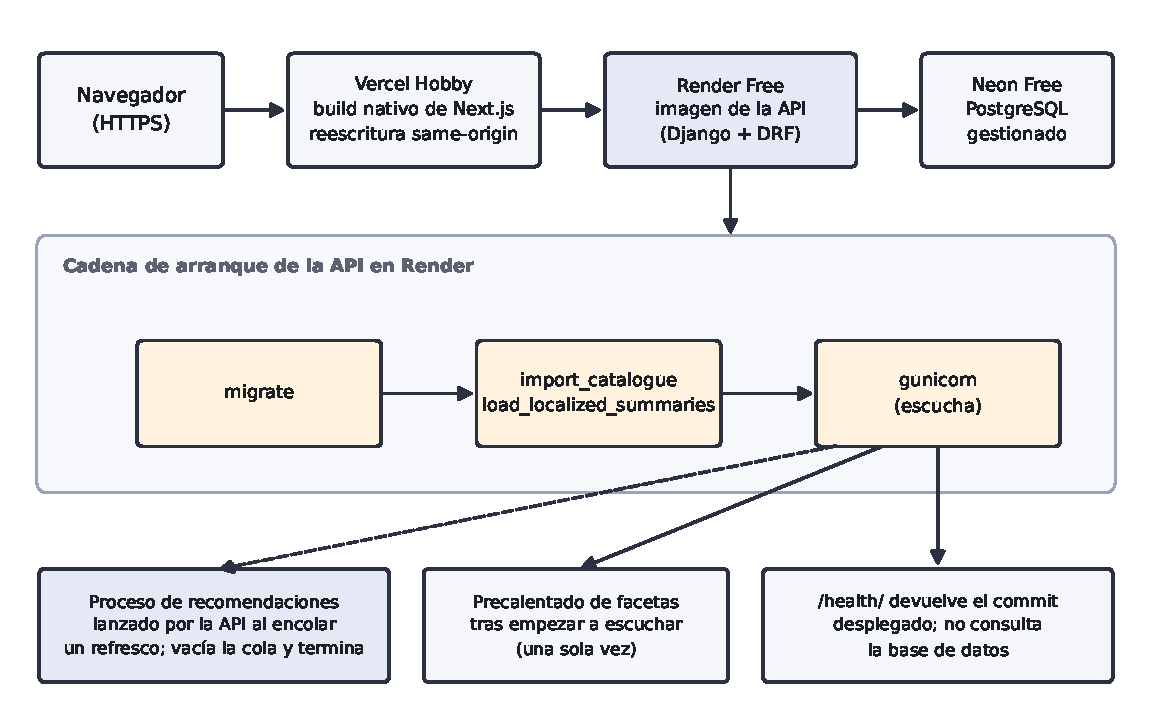
\includegraphics[width=0.92\textwidth]{figures/despliegue-flujo.pdf}
    \caption{Topología de despliegue público y cadena de arranque en Render, en la que cada paso es idempotente y un paso fallido detiene el arranque. Docker Compose local (base de datos, API y frontend) construye las mismas imágenes sin depender de estos tres servicios.}
    \label{fig:despliegue-flujo}
\end{figure}

Docker Compose sigue siendo el entorno reproducible canónico
(Sección~\ref{sec:impl-entorno}). La equivalencia con el
despliegue público es funcional, de versiones, de commit y de datos, no de imagen byte a
byte: el frontend público lo construye Vercel de forma nativa y no ejecuta la imagen de Docker
del frontend, una diferencia de despliegue documentada, no una divergencia de comportamiento.
Si cualquier servicio gratuito duerme, cambia sus términos o desaparece, el entorno local sigue
disponible sin conexión. Los límites conocidos del nivel gratuito se declaran de forma
explícita: el servicio de la API en Render duerme tras quince minutos sin tráfico, de modo que
un visitante puede encontrar un arranque en frío de cerca de un minuto; las cuotas mensuales de
los tres proveedores pueden suspender un servicio, y el nivel gratuito no promete copias de
seguridad ni restauración.

La demostración pública está en vivo desde el 5 de septiembre de 2026, con la prueba de humo en
verde contra la revisión desplegada. En ese despliegue sirve la interfaz anterior al rediseño
contra el corpus curado de ciento cincuenta juegos de Wikidata: el rediseño de la interfaz y el
catálogo a escala real no están en el despliegue público, sino integrados en la rama principal
y ejecutados en el entorno local de Docker Compose. El frontend rediseñado llegó a construirse
en Vercel, pero la base de datos desplegada todavía contiene solo el corpus curado, de modo que
la vista de catálogo da error contra ese despliegue; se revisó esta situación y se decidió
dejar el despliegue público actual como está por ahora, con la demostración ante el tribunal
ejecutándose desde el entorno local reproducible. Conectar el despliegue a datos reales de
internet (cargar el catálogo de IGDB en una base de datos desplegada, aplicar las migraciones
nuevas y ajustar la configuración de hosts y de proxies) queda pospuesto al final del proyecto:
es una decisión registrada, no un defecto pendiente.

Este capítulo ha descrito la construcción, la verificación y el despliegue del sistema. El
capítulo siguiente presenta la evaluación experimental de los algoritmos de recomendación que
se ejecutan sobre él.
